\documentclass[10pt,a4paper]{article}
\usepackage[utf8]{inputenc}
\usepackage{amsmath}
\usepackage{amsfonts}
\usepackage{amssymb}
\usepackage{tabularx,ragged2e,booktabs,caption}
    \newcolumntype{L}{>{\raggedright\arraybackslash}X}
    
\usepackage{listings}
\usepackage[dvipsnames]{xcolor}
\lstset { %
    language=C++,
    backgroundcolor=\color{black!5}, % set backgroundcolor
    keywordstyle=\color{blue!80}\sffamily,%
    commentstyle=\color{OliveGreen},%<==
    %stringstyle=\color{red}% 
    basicstyle=\footnotesize,% basic font setting
}

\usepackage{amsthm}    
\theoremstyle{definition}
\newtheorem{definition}{Definition}[section]

\theoremstyle{plain}
\newtheorem{problem}{Problem}[section]

\theoremstyle{definition}
\newtheorem{solution}{Solution}[section]

\theoremstyle{plain}
\newtheorem{sidenote}{Side Note}[section]

\usepackage{mathtools}
\newcommand{\comp}{^\mathsf{c}}
\newcommand{\powerof}{^{\wedge}}
\newcommand{\der}{\rm{d}}
\DeclarePairedDelimiter\abs{\lvert}{\rvert}%
    
\usepackage[left=2cm,right=2cm,top=2cm,bottom=2cm]{geometry}
\author{Dr Alexander D. Mottram}
\title{Willis Towers Watson Report}

\begin{document}

\maketitle

\section{Expected Attached Files}

First, I'm sorry this document is a bit longer than expected. Most of it is just an aid for me to logical think about and record what I did, and since I started it, I thought I should be complete. I partially solved some of the problems in Excel and MATLAB with some overlap just to compare results. Anyway, I will list here the files and scripts I am attaching as part of this assessment:

\begin{itemize}
\item[•] MarketDataCalibration.xlsx - Excel sheet with analysis for parameter extraction and calibration (tab "Market Data") and also analysis of PayOffs and Option Pricing (tab "PayOff from MC")
\item[•] InterestRateCal\_singlefit.m - MATLAB script that repeated parameter calibration
\item[•] InterestRateCal\_randseed.m - MATLAB script that performed the parameter calibration starting from a set of random seeds
\item[•] InterestRateSim.m - MATLAB script containing Monte Carlo of interest rates
\item[•] OptionPayOffSim.m - MATLAB script that calculates the option pay off using the interest rate Monte Carlo (output of results is included in "PayOff from MC" tab in excel sheet)
\item[•] OptionPricingSim.m - MATLAB script that prices the option using the interest rate Monte Carlo (output of results is included in "PayOff from MC" tab in excel sheet)
\item[•] CalibrationData.mat - Contains the market data provided (necessary to run any of the other MATLAB code)
\end{itemize}

Hopefully I have annotated my code enough that you need not to read any of the following unless you want to further understand the justification behind the choices I made.

\section{Calibration of Parameters}

In Vasicek model given:

\begin{equation}
\der r_r = \gamma \left( \overline{r} - r_t \right) \der t + \sigma \der X_t
\end{equation}

there are three parameters required. But when this stochastic differential equation is used to produce the expectation of the price of a zero coupon the spot interest rate ($r_0$) is also required to produce accurate results. If we are going to fit our model to data of zero coupon bonds priced today with an implicit underlying set of forward rates, then we are working by modelling in a risk-neutral way.

\subsection{Initial Calibration Parameters}

Its preferable to have a set of initial parameters to start any other fitting method from. Considering that zero coupon bonds contain an implicit set of data for future forward interest rates we can use that as a starting point. From Figure \ref{fig:ForwardRates} two regions in the forward rates are observed, a roughly linear region up to Year 2, and then a randomized series of points from Year 4 onwards. 

\begin{figure}[h]
	\centering
	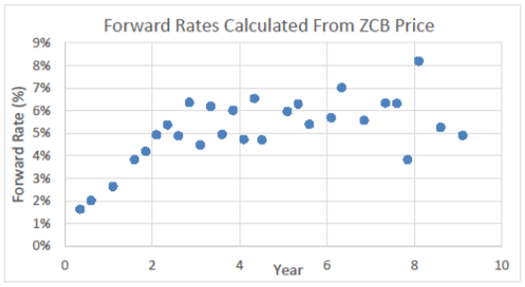
\includegraphics[width=0.7\textwidth]{ForwardRates.png}
	\caption{Forward rates calculates from Zero Coupon Bond data.}
	\label{fig:ForwardRates}
\end{figure}

From this I estimated the four starting parameters as follows:

\begin{itemize}{}
\item $ \overline{r}=5.79\% $ - The mean interest rate is estimated by taking the mean of data points from Year 4 onwards.
\item $\sigma=0.011$ - Assuming that after year 4 the stochastic term is the dominates the variation of the interest rate, the standard deviation of results after Year 4 provides an estimate for $\sigma$.
\item $r_0=0.95\%$ - Upto Year 2 the interest rates follow a seemingly linear pattern so an estimate for the interest rate at $t=0$ can be taken from the intercept of this linear fit with the y axis.
\item $\gamma = 0.74$ - The reversion term of the Vasicek model dominates when the forward interest rate is away from the mean, such as before Year 2. By neglecting the stochastic term a rough estimate for the value of gamma can be calculated between the forward rates.
\end{itemize}

These initial values for the four potential parameters were just found as a starting point and to give rough estimates of the potential ranges for these values.

\subsection{Calibration}

An initial calibration was performed in Excel (Filename: "MarketDataCalibration.xlsx", note that columns are hidden between I and P to save space). Functions of $A(t,T)$ and $B(t,T)$ were calculated and placed into the model for the price of a zero coupon bond $Z(t,T)$:

\begin{equation}
Z(t,T)^{\rm{model}} = e^{\left[ A(t,T)- \left( B(t,T)\cdot r_{t} \right) \right]}.
\end{equation} 

\subsubsection{Justification for Fixing Sigma}
The value of $\sigma$ in the stochastic equation represents the magnitude of the stochastic term and modifies a zero centred unit standard deviation normal distribution. In the pricing model above the effect of this random distribution is only significant when the $\sigma \der X_t > \gamma  \left( \overline{r} - r_t \right) \der t $, at which point the Brownian motion can gain enough "momentum" to escape the reversion term and allow for a path of interest rates that does not revert back to the mean interest rate. This pricing model does not capture the stochastic nature of interest rates though as it is only the expectation, hence fitting of the parameter $\sigma$ is extremely difficult and the solvers in MatLab and Excel tend to set it to $\sigma=0$. Hence I used the value of $\sigma=0.015$ as suggested in the notes which matches to an order of magnitude with the initial value calculated.

\theoremstyle{plain}
\begin{sidenote}{}
If you calculate the forward interest rates from the function for the ZCB model using the equation $R_{F}=-\partial / \partial T \left( ln(Z(0,T)^{\rm{model}}) \right))$, the resultant forward rates contains a term that is proportional to $-\sigma^2$ and only ever reduces the interest rate for values of $\gamma T>2$ (roughly). I suppose this is a problem that arises from the ability of the model to produce negative interest rates, but would be interested to hear a better justification why the general effect of increasing $\sigma$ is to decrease the plateau of the forward interest rate.
\end{sidenote}

\subsubsection{Excel Calibration Results}

After fitting the data in excel I got values of $\gamma=0.77$, $\overline{r}=5.95\%$ and $r_0=0.38\%$. The value for $r_0$ seems somewhat low and is due to the fact that the original spot interest rate quickly becomes irrelevant as the reversion towards the mean interest rate. I'm unsure if the ZCB are based on current day Gilts, but if it where it would put the interest rate near the BoEs current rate of 0.5\%. Either way, when it comes to the Monte Carlo in the next section, the accuracy of the value of $r_0$ becomes less relevant.

\begin{figure}[h]
	\centering
	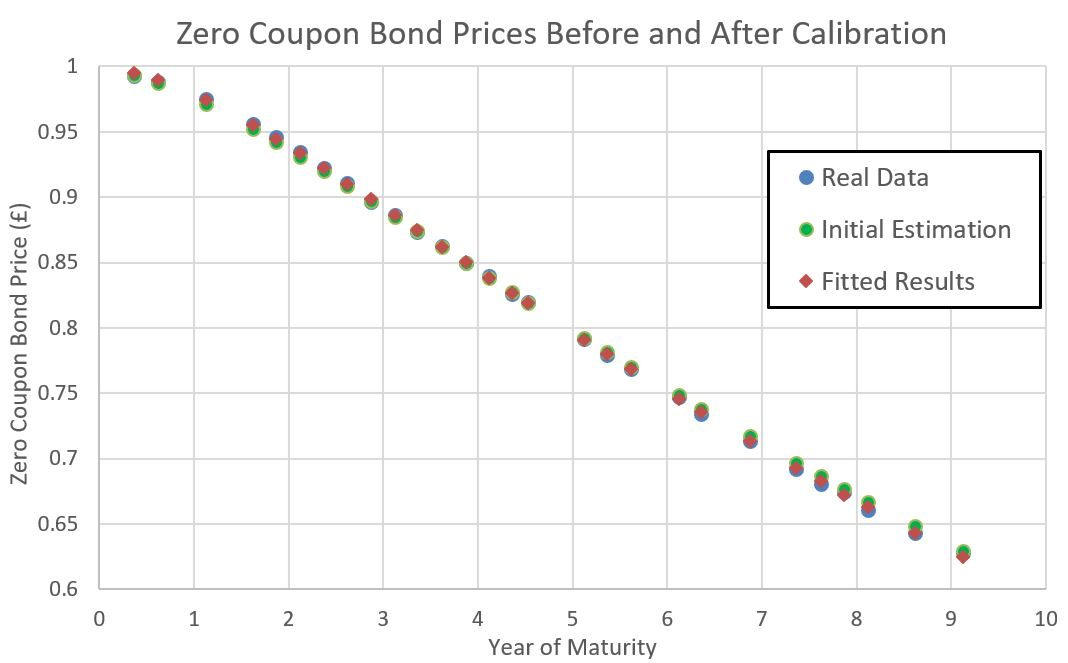
\includegraphics[width=0.8\textwidth]{ExcelCalibrationResults.JPG}
	\caption{Prices of zero coupon bonds, including the real data, the data using the initial calculated parameters and the data fitted using Excel's solver function. Final values after calibration are $\gamma=0.77$, $\overline{r}=5.95\%$ and $r_0=0.38\%$.}
	\label{fig:ExcelCalibration}
\end{figure}

\subsubsection{MATLAB Calibration Results}

To check to see if the solver of MATLAB came out with any different result I replicated the same least squares solving method in MATLAB twice. The first piece of code (FileName: "InterestRateCal\_singlefit.m") performs a least squares fitting starting from the initial parameters shown above. To make sure that the solver wasn't falling into a local minimum a second set of least square fittings was performed (FileName: "InterestRateCal\_randseed.m") on a set of randomised seeds for the initial starting parameters. These seeds were created from normal distributions centred around the initial parameters from above.

\subsection{Final Calibration Results}

Looking at the outcomes from these three different fitting methods, and comparing them to my original values and the suggested values we see that there seems to be a strong consensus for $\overline{r}=6.0\%$. The value for $r_{0}$ tends to come out lower at around 0.37\% than the suggested value likely due to to it's relative weak effect on the overall structure of the price as $T$ increases past the first few initial points.

\begin{center}
\begin{tabular}{c|c|c|c|c|c} 
Parameter & Initial & Excel & MATLAB & MATLAB randseed & Suggested \\ \hline
$\gamma$ & 0.74 & 0.77 & 0.77 & 0.79 & 0.65 \\
$\overline{r}$ & 5.8\% & 6.0\% & 6.0\% & 5.9\% & 6.0\% \\
$r_{0}$ & 0.95\% & 0.38\% & 0.43\% & 0.37\% & 1.0\% \\
\end{tabular}
\end{center}

For the next sections I will use two sets of parameters, first the results from the MATLAB with the random seed generator, and secondly the suggested parameters (in both cases $sigma=0.015$).

\section{Stochastic Monte Carlo Simulation}
I created a Monte Carlo simulation for the interest rates as a function of time (FileName: "InterestRateSim.m") that iterates a small change on the old rate dependant on the Vasicek model equation. Although unnecessary, I made sure that my stochastic term was independent of the time step being used by applying a modified value of $\sigma=\sigma_{yearly}\sqrt{\Delta T}$ where $\Delta T$ is the size of the time step being used (for a yearly simulation this equals one and hence both values of $\sigma$ are identical). The simulation data plots as a histogram of results, and fits a normal distribution to those results to find a mean value of the interest rate for each year.

\captionof{table}{Table of results for average interest rate of 1000 simulation paths with yearly time steps for two set of parameters.}
\begin{center}
\begin{tabular}{c|c|c}
Year & Param = MATLAB randseed & Param = Suggested \\ \hline
0 & 0.53 \% & 1.00 \% \\
1 & 4.80 \% & 4.21 \% \\
2 & 5.63 \% & 5.39 \% \\
3 & 5.80 \% & 5.84 \% \\
4 & 6.00 \% & 6.02 \% \\
5 & 5.90 \% & 6.03 \% \\
\end{tabular}
\end{center}

The results from the simulation show that after 2 years the difference in interest rates between the MATLAB randomly seeded and solved parameters and the suggested parameters are very similar.

\section{Pricing the Option}

We have an option where the underlying asset is the price of a bond with maturity date $T_{2}$. Hopefully, if I understand correctly, this is the price that would be simulated for a bond starting at time $T_{1}$ and maturing at $T_{2}$. I have calculated this price using two methods, first by just taking the average interest rate and working out the price of bonds starting purchased at Year X and expiring at Year Y (included in File "MarketDataCalibration.xlsx" in tab "PayOff from MC"). The results form this first set of calculations can be seen in the top section of Figure \ref{fig:PayOffandPrice}.


\begin{figure}[h]
	\centering
	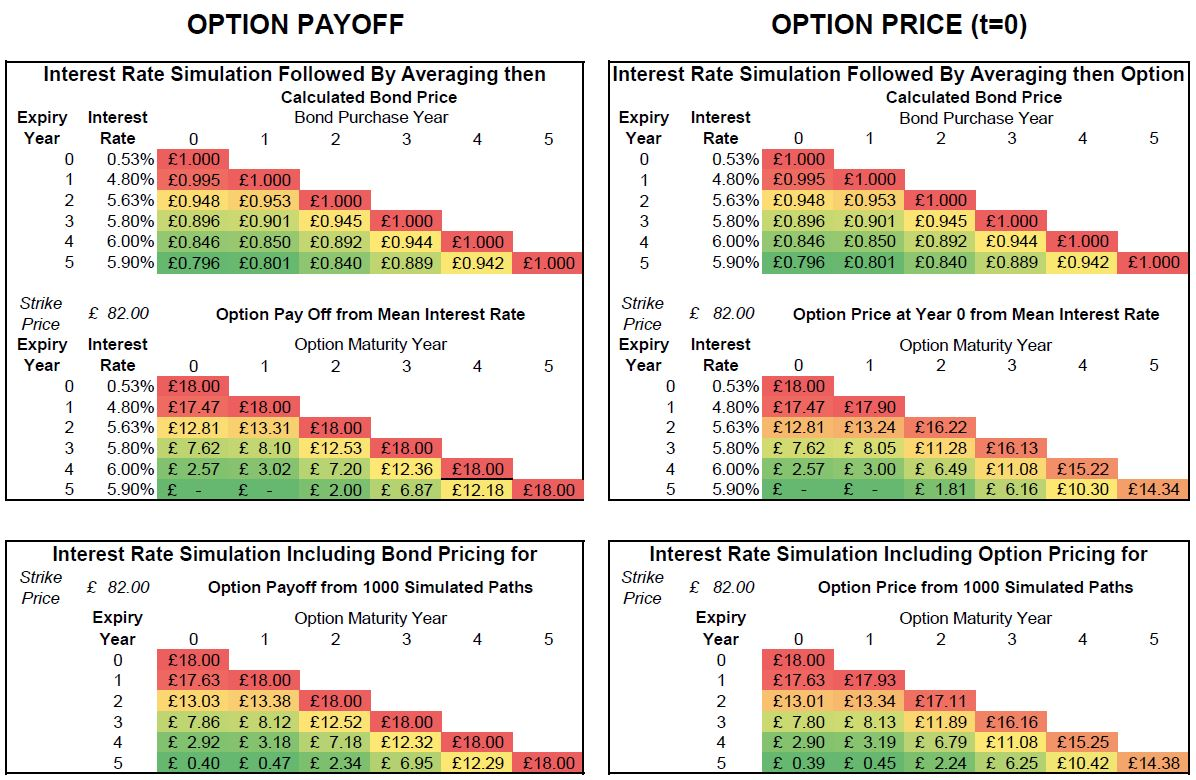
\includegraphics[width=1\textwidth]{PayOffandPrice.JPG}
	\caption{PayOffs (left column) and option pricing at $t=0$ (right column) calculated by using average values for the interest rate (top) and 1000 simulated pathways (bottom).}
	\label{fig:PayOffandPrice}
\end{figure}

The problem with using the average interest rate is that there are potential paths that would have produced a PayOff that aren't included because the mean price is lower than the cut off of £82 (e.g. for purchase year 1, maturity year 5). So I created a new simulation in MATLAB by adding a small piece of code to the end of my interest rate price Monte Carlo simulation (FileName: "OptionPayOffSim.m"). The extra code basically analyses the expected payout for each path , and then takes a mean of these payouts, as opposed to averaging the interest rates first. The results of these simulations are given in Figure \ref{fig:PayOffandPrice} (bottom left).

To price the payoffs we have to take into account the time value aspect by reducing the payoff by $e^{-r_{year}}$ for each year before the maturity date of the bond. The results of this are included in the right hand side of Figure \ref{fig:PayOffandPrice} using the two methods of averaging simulated interest rates (top) and averaging simulated option prices (bottom). The code for option pricing is included in FileName: "OptionPricingSim.m". Therefore, the price for $T_{1}=2$, $T_{2}=5$ and $K=$£82 is £2.24.

\section{Model Parameters and Option Pricing}
Finally how do the parameters affect the option pricing. First, any parameter that causes a decrease in bond price will move the distribution of potential bond prices lower and hence reduce the amount of potential paths which will pay out. This means a decrease in bond prices will lead to a decrease in the price of the option.

\begin{itemize}
\item $\gamma$ - An increase in the rate of reversion will decrease option prices as the interest rate will revert to the mean quicker, hence reducing prices to buy an underlying bond. There is an exception though, if the rate of reversion becomes to large it will cause unstable oscillations in the system causing alternately massive negative and positive values of interest rates between concurrent time steps (this is hopefully an "unreal" situation though).
\item $\overline{r}$ - An increase in the mean interest rate will lead to a decrease in the option price since the price of a bond will be lower.
\item $r_{0}$ - Increasing the instantaneous spot interest rate will decrease the price of the underlying bond decreasing the price of the option. This is the same mechanism as for the mean interest rate, but since the instantaneous spot rate becomes less important as time progress it is most important in bonds close to their expiry date.
\item $\sigma$ - Increasing sigma increases the stochastic term in the bond price and introduces greater variation and more potential paths where bond prices are higher (or at least higher to a greater degree due to a wider spread in the potential bond prices). It also increases the extreme lows, but since this is an option and not a forward contract the risk of loss is limited. This therefore increases the price of the option.
\end{itemize}



\end{document}